\documentclass[10pt,twocolumn]{article}

\usepackage[margin=0.72in]{geometry}
\usepackage{booktabs}
\usepackage{graphicx}
\usepackage{tabularx}
\usepackage{array}
\usepackage{caption}
\usepackage{microtype}
\usepackage{cite}
\usepackage{tikz}
\usetikzlibrary{arrows.meta,positioning}
\usepackage[hidelinks]{hyperref}

% Submission checklist: replace article class with official COMPAS template.
% Submission checklist: verify dataset citation/version/license.
% Submission checklist: check final PDF metadata for double-blind compliance.
% Submission checklist: confirm page limit and bibliography style.

\setlength{\textfloatsep}{8pt plus 2pt minus 2pt}
\setlength{\floatsep}{8pt plus 2pt minus 2pt}
\setlength{\intextsep}{8pt plus 2pt minus 2pt}
\captionsetup{font=small}
\newcolumntype{L}[1]{>{\raggedright\arraybackslash}p{#1}}
\newcolumntype{C}[1]{>{\centering\arraybackslash}p{#1}}
\newcolumntype{Y}{>{\raggedright\arraybackslash}X}

\newcommand{\authorblock}[2]{%
    \begin{minipage}[t]{0.42\textwidth}
        \centering
        {\normalsize\bfseries #1\par}
        \vspace{0.15em}
        {\footnotesize\texttt{#2}\par}
        \vspace{0.25em}
        {\footnotesize Department of Computer Science\par}
        {\footnotesize Faculty of Science and Technology\par}
        {\footnotesize American International University-Bangladesh\par}
        {\footnotesize Dhaka, Bangladesh\par}
    \end{minipage}
}

\newcommand{\papertitleblock}{%
\begin{center}
{\LARGE\bfseries Communication-Efficient Federated Brain Tumor MRI\\[-0.2em]
Classification with EfficientNet-B0\par}
\vspace{1.0em}
\authorblock{Nidan Alam}{22-47046-1@student.aiub.edu}
\hfill
\authorblock{Abu Jafar Sisty}{22-49133-3@student.aiub.edu}
\end{center}
\vspace{0.65em}
}

\begin{document}
\twocolumn[
\papertitleblock
]

\begin{abstract}
Federated learning can support collaborative medical image model training without centralizing image data in the simulated FL protocol, but communication cost and evaluation reliability remain practical concerns. This paper studies four-class brain tumor MRI classification under a cluster-aware duplicate-controlled split and compares compact and heavier convolutional backbones using simulated clients. The experiments use 5,040 training images, 720 validation images, and 1,440 test images, with duplicate and near-duplicate image clusters assigned to a single split. A centralized screening stage selected EfficientNet-B0 because it achieved the strongest validation macro-F1 among the tested backbones and reached 97.71\% test accuracy and 97.71\% test macro-F1. In 20-round federated learning with four virtual clients, EfficientNet-B0 achieved 97.64\% accuracy and 97.64\% macro-F1 in the Non-IID setting, compared with 97.22\% accuracy and 97.23\% macro-F1 for ResNet50. EfficientNet-B0 reduced total full-state communication from 14,385.65 MB to 2,474.84 MB, corresponding to approximately 82.8\% lower communication. These results suggest that a compact backbone can preserve test performance while substantially reducing communication in this simulated experimental setting.
\end{abstract}

\section{Introduction}
Brain tumor MRI classification is widely used as a public benchmark for medical image classification and federated learning studies \cite{nickparvar_brain_tumor_mri,bentemessek2025brain,khatoon2026resnet50,ghanta2025federated}. These datasets are useful because they provide accessible four-class classification tasks, but public image collections also make evaluation discipline especially important. Duplicate or patient-overlapping MRI slices across training and testing sets can cause data leakage and optimistically biased performance estimates \cite{melo2026exploiting,siam2026brain,naseer2026medfl}. A high test score is less informative if related slices appear on both sides of the split.

Federated learning (FL) addresses a different constraint. It trains models across clients without centralizing raw image data in the simulated protocol, which is attractive for medical imaging settings where data movement is restricted \cite{rieke2020future,sharma2025privacy,mastoi2025explainable}. Standard FL should still be described carefully: transmitted model updates can leak information, and FL alone should not be treated as complete privacy or regulatory compliance \cite{rieke2020future,naseer2026medfl}. In addition, repeated exchange of high-dimensional model states creates communication overhead, which can be a bottleneck in bandwidth-constrained FL settings \cite{mcmahan2017fedavg,radhika2026communication,zhou2022communication}.

This work evaluates a compact federated brain tumor MRI classifier using a cluster-aware duplicate-controlled split and a 20-round simulated FL setup. The central question is practical: can EfficientNet-B0 provide comparable classification performance to a larger ResNet50 baseline while reducing full-state communication cost under the same FL schedule? The contribution is an empirical, audit-informed comparison under virtual clients, not evidence of clinical deployment readiness or full privacy compliance.

The contributions are:
\begin{itemize}
    \raggedright
    \setlength{\itemsep}{0.15em}
    \setlength{\parsep}{0pt}
    \item \textbf{Duplicate-controlled evaluation:} a cluster-aware split for reliable evaluation of four-class brain tumor MRI classification.
    \item \textbf{Backbone screening:} a centralized selection step that identifies EfficientNet-B0 as a compact high-performing model.
    \item \textbf{Federated comparison:} a 20-round evaluation showing EfficientNet-B0 achieves similar or slightly better Non-IID performance than ResNet50 with substantially lower full-state communication.
\end{itemize}

\section{Related Work}
\subsection{Federated Learning for Medical Imaging}
FedAvg remains the standard starting point for FL: clients train local models and a server aggregates their updates using sample-count weighting \cite{mcmahan2017fedavg}. FedProx extends this framework by adding a proximal term during local optimization, making it a common baseline for heterogeneous FL because it can reduce local model divergence under Non-IID data \cite{li2020fedprox,ghanta2025federated}. Heterogeneous Non-IID client distributions can cause client drift, training instability, and reduced global model performance, especially when labels or acquisition conditions differ across sites \cite{ghanta2025federated,xu2023federated,naseer2026medfl}.

Medical imaging studies use FL to explore collaborative training when raw image sharing is undesirable or restricted \cite{rieke2020future}. Recent work has applied FL to glioma detection, four-class brain tumor MRI classification, and segmentation or analysis tasks across distributed or multi-center settings \cite{sharma2025privacy,mastoi2025explainable,saraswat2026hybrid,wakili2025twinsegnet}. These studies motivate FL for medical image analysis, but they also show why controlled simulations need careful wording. Simulated client partitions do not replace external validation across independent clinical sites, and a four-client split from one public dataset cannot capture scanner, protocol, population, and governance differences seen in real hospital networks \cite{naseer2026medfl,xu2023federated}.

\subsection{Brain Tumor MRI Classification and Dataset Reliability}
The Nickparvar brain tumor MRI dataset is a common public image classification source for glioma, meningioma, no tumor, and pituitary categories \cite{nickparvar_brain_tumor_mri}. ResNet50-based studies and comparative CNN experiments have helped establish this dataset family as a practical benchmark for tumor classification pipelines \cite{he2016resnet,bentemessek2025brain,khatoon2026resnet50}. FL studies have also used brain tumor MRI tasks to evaluate FedAvg, FedProx, lightweight backbones, and explainable medical imaging models \cite{ghanta2025federated,sharma2025privacy,mastoi2025explainable}.

At the same time, dataset reliability is a recurring concern. Melo et al. report duplicate removal using SHA-256 before FL splitting, and Siam and Khan emphasize patient-wise or cluster-aware splitting for brain tumor MRI FL simulations \cite{melo2026exploiting,siam2026brain}. These points are directly relevant to public MRI collections, where slices may be visually similar or duplicated across folders. Our split therefore groups exact duplicates, pixel duplicates, and conservative near-duplicate image families before assigning images to train, validation, or test partitions. This reduces a specific evaluation risk, although it does not remove all public dataset bias.

\subsection{Communication and Backbone Efficiency}
Communication cost is built into FL. Each round exchanges model information between clients and the server, and larger backbones increase the payload when full states are transmitted \cite{mcmahan2017fedavg}. Prior medical FL studies have explored communication-aware training through sparsification, quantization, upload constraints, or other efficiency mechanisms \cite{radhika2026communication,aniket2025cfl,zhou2022communication,das2026federated}. A complementary path is to choose a compact backbone before FL begins.

ResNet50 is a strong and familiar visual baseline, but it is heavier than compact architectures in our implementation \cite{he2016resnet,bentemessek2025brain,khatoon2026resnet50}. EfficientNet uses compound scaling to balance depth, width, and input resolution, and EfficientNet-B0 has been used as a lightweight backbone in medical FL settings \cite{tan2019efficientnet,abubakr2026explainable}. The gap addressed here is narrower than proposing a new algorithm: we combine cluster-aware duplicate-controlled evaluation, centralized backbone screening, a direct EfficientNet-B0 versus ResNet50 comparison under the same 20-round simulated FL setting, and explicit full-state upload/download accounting.

\section{Methodology}
The experimental workflow is organized into four stages: constructing a duplicate-controlled split from the public MRI dataset, screening candidate backbones under centralized training, simulating IID and label-skewed federated client partitions, and comparing final accuracy and full-state communication cost. Figure~\ref{fig:pipeline} shows this end-to-end pipeline.

\begin{figure*}[t]
\centering
\resizebox{\textwidth}{!}{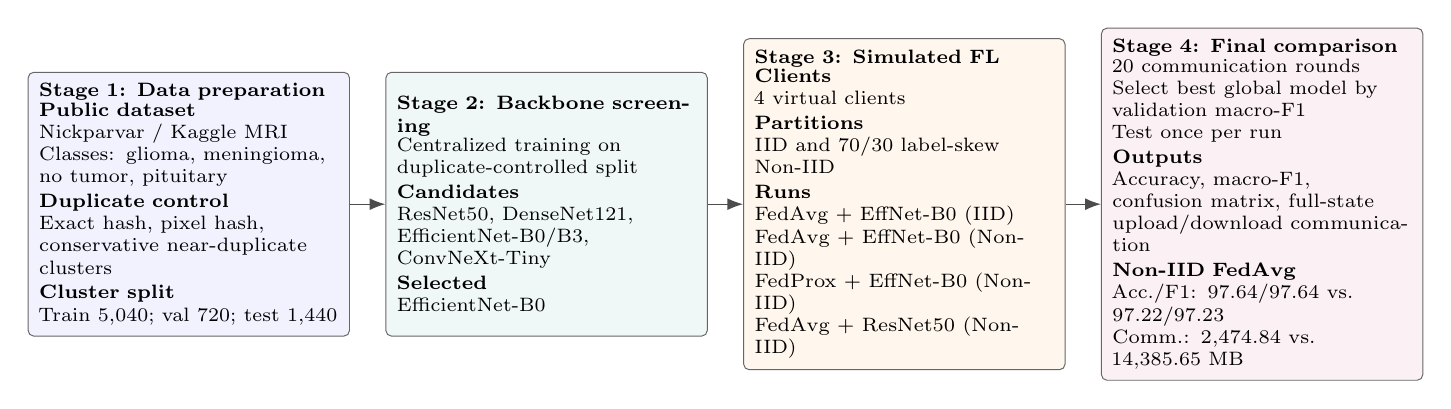
\begin{tikzpicture}[
  font=\scriptsize,
  stage/.style={
    draw=black!60,
    rounded corners=2pt,
    line width=0.35pt,
    align=left,
    inner sep=4pt,
    text width=3.8cm,
    minimum height=3.35cm
  },
  arrow/.style={-{Latex[length=2mm]}, draw=black!70, line width=0.45pt},
  stagetitle/.style={font=\bfseries\scriptsize}
]
\node[stage, fill=blue!5] (data) {
  \textbf{Stage 1: Data preparation}\\[-1pt]
  \textbf{Public dataset}\\
  Nickparvar / Kaggle MRI\\
  Classes: glioma, meningioma,\\
  no tumor, pituitary\\[1pt]
  \textbf{Duplicate control}\\
  Exact hash, pixel hash,\\
  conservative near-duplicate clusters\\[1pt]
  \textbf{Cluster split}\\
  Train 5,040; val 720; test 1,440
};

\node[stage, fill=teal!6, right=0.45cm of data] (screen) {
  \textbf{Stage 2: Backbone screening}\\[-1pt]
  Centralized training on\\
  duplicate-controlled split\\[1pt]
  \textbf{Candidates}\\
  ResNet50, DenseNet121,\\
  EfficientNet-B0/B3,\\
  ConvNeXt-Tiny\\[1pt]
  \textbf{Selected}\\
  EfficientNet-B0
};

\node[stage, fill=orange!7, right=0.45cm of screen] (fl) {
  \textbf{Stage 3: Simulated FL}\\[-1pt]
  \textbf{Clients}\\
  4 virtual clients\\[1pt]
  \textbf{Partitions}\\
  IID and 70/30 label-skew\\
  Non-IID\\[1pt]
  \textbf{Runs}\\
  FedAvg + EffNet-B0 (IID)\\
  FedAvg + EffNet-B0 (Non-IID)\\
  FedProx + EffNet-B0 (Non-IID)\\
  FedAvg + ResNet50 (Non-IID)
};

\node[stage, fill=purple!6, right=0.45cm of fl] (out) {
  \textbf{Stage 4: Final comparison}\\[-1pt]
  20 communication rounds\\
  Select best global model by\\
  validation macro-F1\\
  Test once per run\\[1pt]
  \textbf{Outputs}\\
  Accuracy, macro-F1,\\
  confusion matrix, full-state\\
  upload/download communication\\[1pt]
  \textbf{Non-IID FedAvg}\\
  Acc./F1: 97.64/97.64 vs.\\
  97.22/97.23\\
  Comm.: 2,474.84 vs. 14,385.65 MB
};

\draw[arrow] (data.east) -- (screen.west);
\draw[arrow] (screen.east) -- (fl.west);
\draw[arrow] (fl.east) -- (out.west);
\end{tikzpicture}
}
\caption{Pipeline overview: public dataset, duplicate-controlled split, centralized screening, simulated FL evaluation, and final metric/communication comparison.}
\label{fig:pipeline}
\end{figure*}

\subsection{Dataset and Cluster-Aware Duplicate-Controlled Split}
The experiments use a four-class brain tumor MRI dataset with glioma, meningioma, no tumor, and pituitary classes \cite{nickparvar_brain_tumor_mri}. Instead of relying on the original folder split directly, all available images were pooled and assigned to a cluster-aware duplicate-controlled split. Images were represented as graph nodes, with edges connecting exact SHA-256 duplicates, pixel-level duplicates after RGB resizing to 224 by 224, and conservative same-class near-duplicates based on perceptual hashing and structural similarity. Connected components defined image clusters, and each cluster was assigned to exactly one final split. This follows the motivation in recent duplicate-removal and patient-wise partitioning work for brain tumor MRI FL \cite{melo2026exploiting,siam2026brain}.

The resulting split contains 5,040 training images, 720 validation images, and 1,440 test images. Each split is class balanced: the training set contains 1,260 images per class, the validation set 180 images per class, and the test set 360 images per class. A post-split duplicate check found no exact, pixel-level, or conservative near-duplicate overlaps across train, validation, and test splits. The split improves internal evaluation reliability, but it does not create an external cohort or guarantee patient-level independence beyond the evidence available in the public image collection.

Table~\ref{tab:split-counts} reports the resulting class-balanced train, validation, and test partitions.

\begin{table}[t]
\centering
\caption{Class distribution in the cluster-aware duplicate-controlled split.}
\label{tab:split-counts}
\scriptsize
\setlength{\tabcolsep}{2pt}
\begin{tabular*}{\columnwidth}{@{\extracolsep{\fill}}lrrrrr@{}}
\toprule
Split & Glioma & Meningioma & No tumor & Pituitary & Total \\
\midrule
Train & 1,260 & 1,260 & 1,260 & 1,260 & 5,040 \\
Validation & 180 & 180 & 180 & 180 & 720 \\
Test & 360 & 360 & 360 & 360 & 1,440 \\
\bottomrule
\end{tabular*}
\end{table}

\subsection{Centralized Backbone Screening}
Before running FL, a centralized benchmark compared candidate ImageNet-pretrained backbones using the cluster-aware split. The screening used 224 by 224 inputs, AdamW optimization, early stopping on validation macro-F1, and test evaluation only for the selected model. ResNet50 served as a heavier baseline backbone \cite{he2016resnet}, while EfficientNet-B0 represented a compact alternative motivated by compound scaling and prior medical FL use \cite{tan2019efficientnet,abubakr2026explainable}.

EfficientNet-B0 with learning rate 0.0003 achieved the best validation macro-F1 among the tested runs. The selected centralized model reached 97.71\% test accuracy and 97.71\% test macro-F1. This screening step was used to choose the compact backbone for the final FL comparison, rather than selecting a federated model after looking at the FL test set.

\subsection{Simulated Federated Learning Setup}
The final FL experiments used four simulated clients, 20 communication rounds, three local epochs per round, batch size 32, AdamW, learning rate 0.0003, weight decay 0.0001, and seed 42. All client partitions were simulated from the same dataset; no real hospital or institutional client deployment was used. The IID partition split each class approximately evenly across virtual clients. The Non-IID partition was a controlled 70/30 label-skew split with one dominant class per client, assigning 70\% of each class to its dominant client and distributing the remainder across the other clients. This design stresses label imbalance but does not represent real institutional heterogeneity in scanner protocols, acquisition sites, or patient populations.

For FedAvg, the server aggregated full model state dictionaries using sample-count-weighted averaging \cite{mcmahan2017fedavg}:
\begin{equation}
    w^{(t+1)} = \sum_{k=1}^{K} \frac{n_k}{\sum_j n_j} w_k^{(t+1)},
\end{equation}
where $K$ is the number of clients, $n_k$ is the number of samples on client $k$, and $w_k^{(t+1)}$ is the locally updated model state. FedProx used the same aggregation rule but added the proximal term described by Li et al. during local optimization \cite{li2020fedprox}. It is included as a heterogeneous-FL baseline, not because it improved the final result in this experiment.

\subsection{Communication Accounting}
Communication cost was computed from the actual full \texttt{state\_dict} tensor bytes transmitted for every server-to-client download and every client-to-server upload. Thus, for a model with state size $S$, $K$ clients, and $R$ rounds, total communication is $2SKR$. This accounting intentionally reflects full-state communication rather than trainable-only parameters, gradients, sparse updates, compressed updates, or network latency. It therefore isolates the payload effect of backbone choice, which prior work identifies as one part of the broader medical FL communication bottleneck \cite{radhika2026communication,zhou2022communication,das2026federated}.

\section{Results and Discussion}
\subsection{Centralized Model Selection}
The centralized screening stage was used only to choose a backbone before the final FL experiments. EfficientNet-B0 achieved the best validation macro-F1 among the tested configurations and reached 97.71\% test accuracy and 97.71\% test macro-F1 on the cluster-aware duplicate-controlled split. This result does not imply that EfficientNet-B0 is universally preferable, but it provides a measured reason to compare it against ResNet50 in the fixed FL protocol.

\subsection{20-Round Federated Results}
Because related studies differ in class definitions, datasets, client counts, heterogeneity settings, and evaluation protocols, Table~\ref{tab:context-comparison} is intended as a \textit{contextual comparison rather than a direct leaderboard}.

\begin{table*}[t]
\centering
\caption{Contextual comparison with related federated brain tumor MRI studies.}
\label{tab:context-comparison}
\scriptsize
\setlength{\tabcolsep}{2.5pt}
\renewcommand{\arraystretch}{1.08}
\begin{tabularx}{\textwidth}{@{}L{1.75cm}Y Y L{1.85cm}Y Y L{1.7cm}@{}}
\toprule
Study & Task & FL setup & Model & Reported result & Communication reported & Comparable? \\
\midrule
Mastoi et al. 2025 \cite{mastoi2025explainable} & Four-class brain tumor MRI classification & 10 clients, 50 rounds & GoogLeNet + FL + XAI & 94.0\% accuracy & No full-state accounting & Partial \\
Ghanta et al. 2025 \cite{ghanta2025federated} & Four-class brain tumor MRI classification & 4 clients, FedProx, IID and extreme Non-IID & ResNet50 & 97.71\% IID; 87.19\% extreme Non-IID & Not primary focus & Partial \\
This work & Four-class brain tumor MRI classification & 4 virtual clients, 20 rounds, IID and 70/30 label-skew Non-IID & EfficientNet-B0 & 97.92\% IID; 97.64\% Non-IID & Yes; full-state upload/download; 2,474.84 MB for EfficientNet-B0 Non-IID & Reference row \\
\bottomrule
\end{tabularx}
\end{table*}

Binary glioma-detection studies are discussed in Related Work but excluded from the main comparison table because their task setting is not directly comparable to four-class brain tumor MRI classification.

Table~\ref{tab:fl-results} summarizes the final 20-round FL results. FedAvg EfficientNet-B0 achieved 97.92\% accuracy in the IID setting and 97.64\% accuracy in the Non-IID setting. FedProx with EfficientNet-B0 produced essentially the same Non-IID test performance as FedAvg, with 97.64\% accuracy and 97.64\% macro-F1. For this split and hyperparameter configuration, the FedProx proximal term did not meaningfully improve the final test result, despite its role as a common baseline for heterogeneous FL \cite{li2020fedprox,ghanta2025federated}.

\begin{table*}[t]
\centering
\caption{Final 20-round federated test results. All runs use four simulated clients and select the best global model by validation macro-F1.}
\label{tab:fl-results}
\scriptsize
\setlength{\tabcolsep}{3.5pt}
\begin{tabular*}{\textwidth}{@{\extracolsep{\fill}}llcrrrrrr@{}}
\toprule
Method & Backbone & Partition & Best & Acc. (\%) & Macro-F1 (\%) & Params (M) & State (MB) & Comm. (MB) \\
\midrule
FedAvg & EfficientNet-B0 & IID & 20 & 97.92 & 97.92 & 4.01 & 15.47 & 2,474.84 \\
FedAvg & EfficientNet-B0 & Non-IID & 20 & 97.64 & 97.64 & 4.01 & 15.47 & 2,474.84 \\
FedProx & EfficientNet-B0 & Non-IID & 20 & 97.64 & 97.64 & 4.01 & 15.47 & 2,474.84 \\
FedAvg & ResNet50 & Non-IID & 15 & 97.22 & 97.23 & 23.52 & 89.91 & 14,385.65 \\
\bottomrule
\end{tabular*}
\end{table*}

Figure~\ref{fig:convergence} shows validation macro-F1 across communication rounds. EfficientNet-B0 reached high validation macro-F1 early and remained competitive through round 20. ResNet50 improved over training but showed lower validation macro-F1 than the EfficientNet-B0 runs for most rounds. These curves should be interpreted as validation behavior under a single fixed split and seed, not as a broad convergence guarantee.

\begin{figure*}[t]
\centering
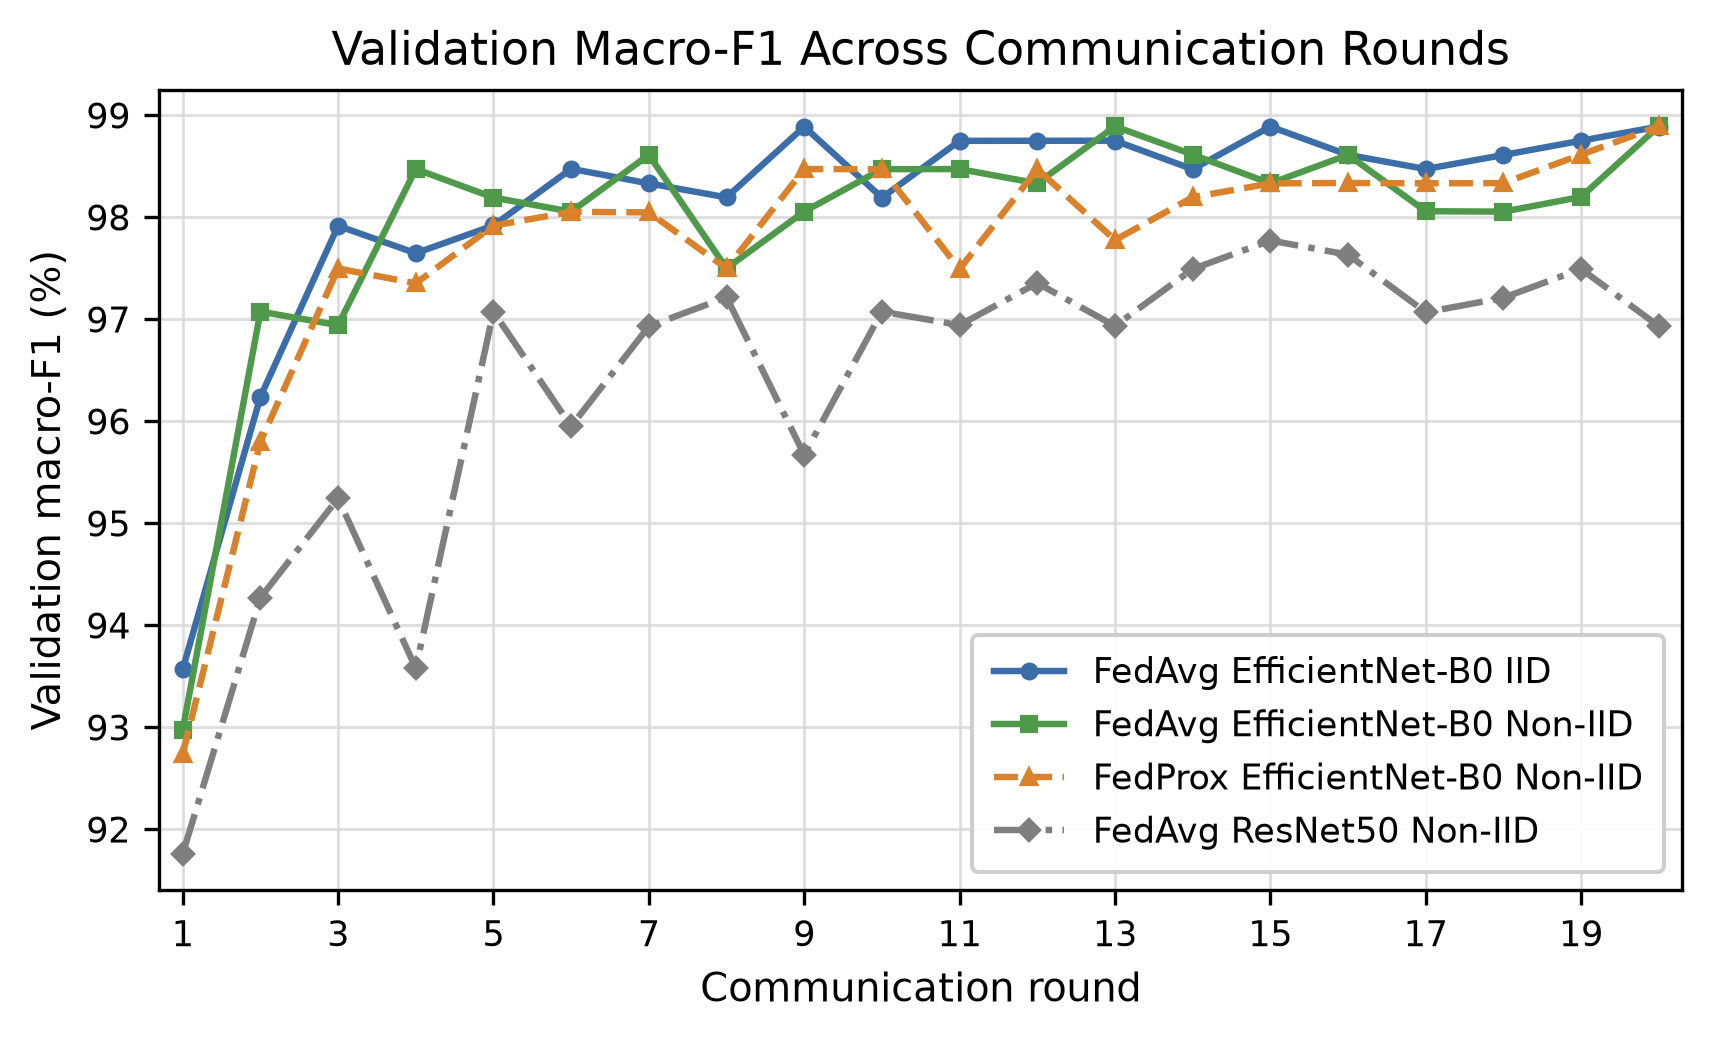
\includegraphics[width=0.78\textwidth]{figures/fig_convergence_val_macro_f1.png}
\caption{Validation macro-F1 across 20 communication rounds for the final FL runs.}
\label{fig:convergence}
\end{figure*}

\subsection{Communication Comparison}
The primary communication comparison is between FedAvg EfficientNet-B0 Non-IID and FedAvg ResNet50 Non-IID, because both use the same simulated client count, round count, optimizer, local epochs, and partition type. Under the same 4-client, 20-round Non-IID FedAvg setting, EfficientNet-B0 achieved 97.64\% accuracy and 97.64\% macro-F1, compared with 97.22\% accuracy and 97.23\% macro-F1 for ResNet50. EfficientNet-B0 reduced total communication from 14,385.65 MB to 2,474.84 MB, approximately 82.8\% lower.

\begin{table}[t]
\centering
\caption{Communication comparison under the same 4-virtual-client, 20-round Non-IID FedAvg setting.}
\label{tab:comm}
\scriptsize
\setlength{\tabcolsep}{3pt}
\begin{tabular}{@{}lrrrr@{}}
\toprule
Backbone & State & Total & Ratio & Red. \\
\midrule
EfficientNet-B0 & 15.47 & 2,474.84 & 0.172 & 82.8 \\
ResNet50 & 89.91 & 14,385.65 & 1.000 & 0.0 \\
\bottomrule
\end{tabular}
\vspace{1mm}
\caption*{\scriptsize State and total communication are reported in MB; Red. denotes communication reduction relative to ResNet50.}
\end{table}

\begin{figure}[t]
\centering
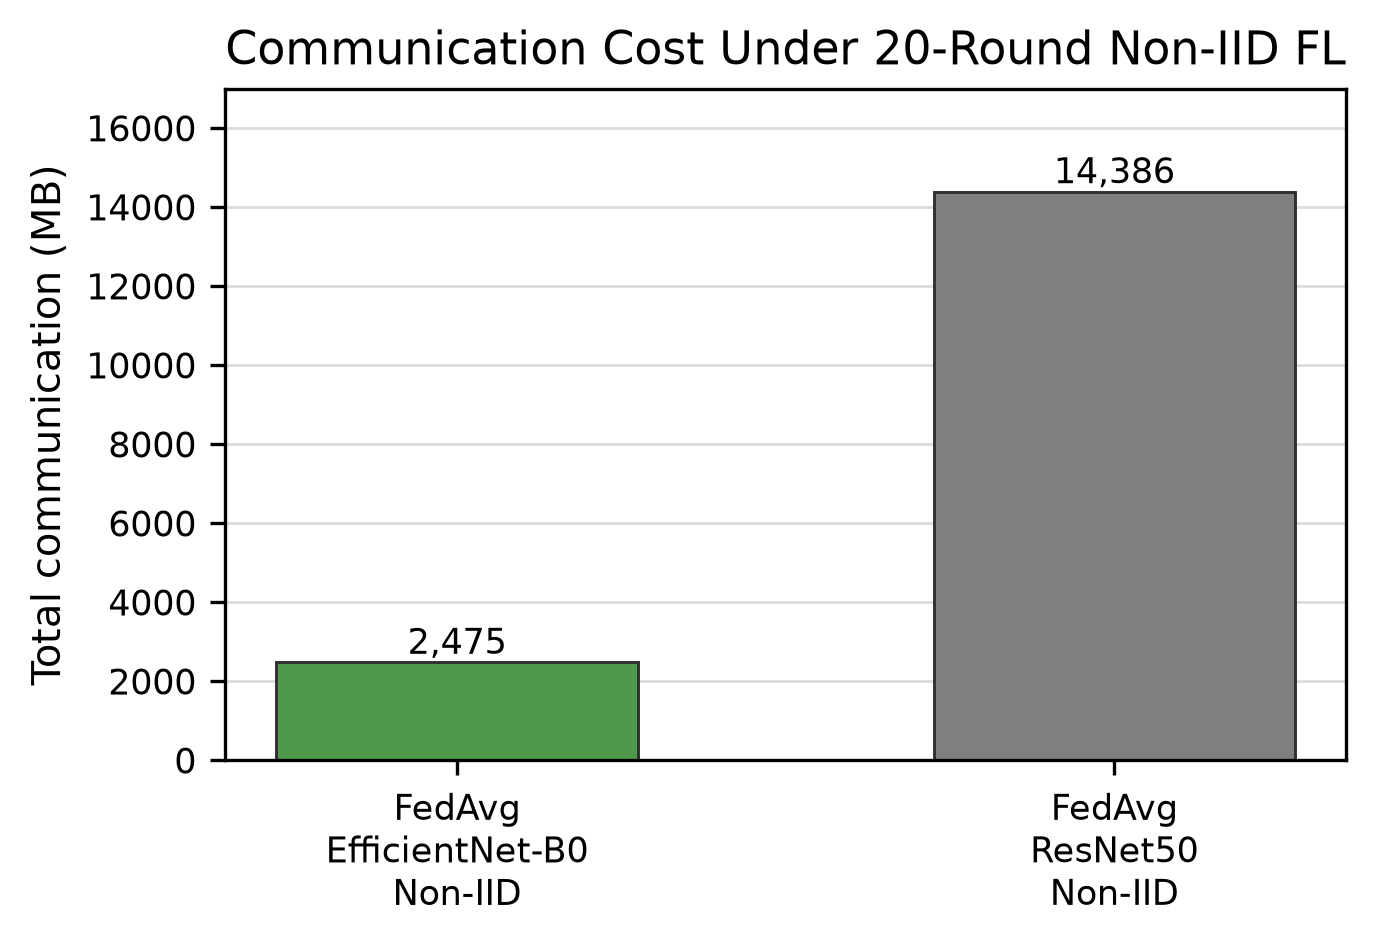
\includegraphics[width=\columnwidth]{figures/fig_main_communication_comparison.png}
\caption{Total full-state communication under 20-round Non-IID FedAvg.}
\label{fig:comm}
\end{figure}

EfficientNet-B0's compound scaling balances depth, width, and resolution, allowing the model to retain useful spatial representations with a smaller parameter footprint \cite{tan2019efficientnet}. ResNet50 remains a strong residual baseline \cite{he2016resnet}, but it is heavier in our implementation: 23.52M parameters and an 89.91 MB state dictionary, compared with 4.01M parameters and a 15.47 MB state dictionary for EfficientNet-B0. Because full model states are exchanged in every FL upload and download, the architectural benefit in this setting is not a large accuracy gain, but a better accuracy--communication trade-off.

\subsection{Class-Wise Behavior}
Figure~\ref{fig:cm} presents the Non-IID FedAvg EfficientNet-B0 confusion matrix. The model classified most test images correctly across all four classes. The largest off-diagonal counts were between glioma and meningioma and between meningioma and pituitary, which are plausible error modes for visual classification models on MRI slices. These results support the aggregate macro-F1 score but should not be treated as clinical validation.

\begin{figure}[t]
\centering
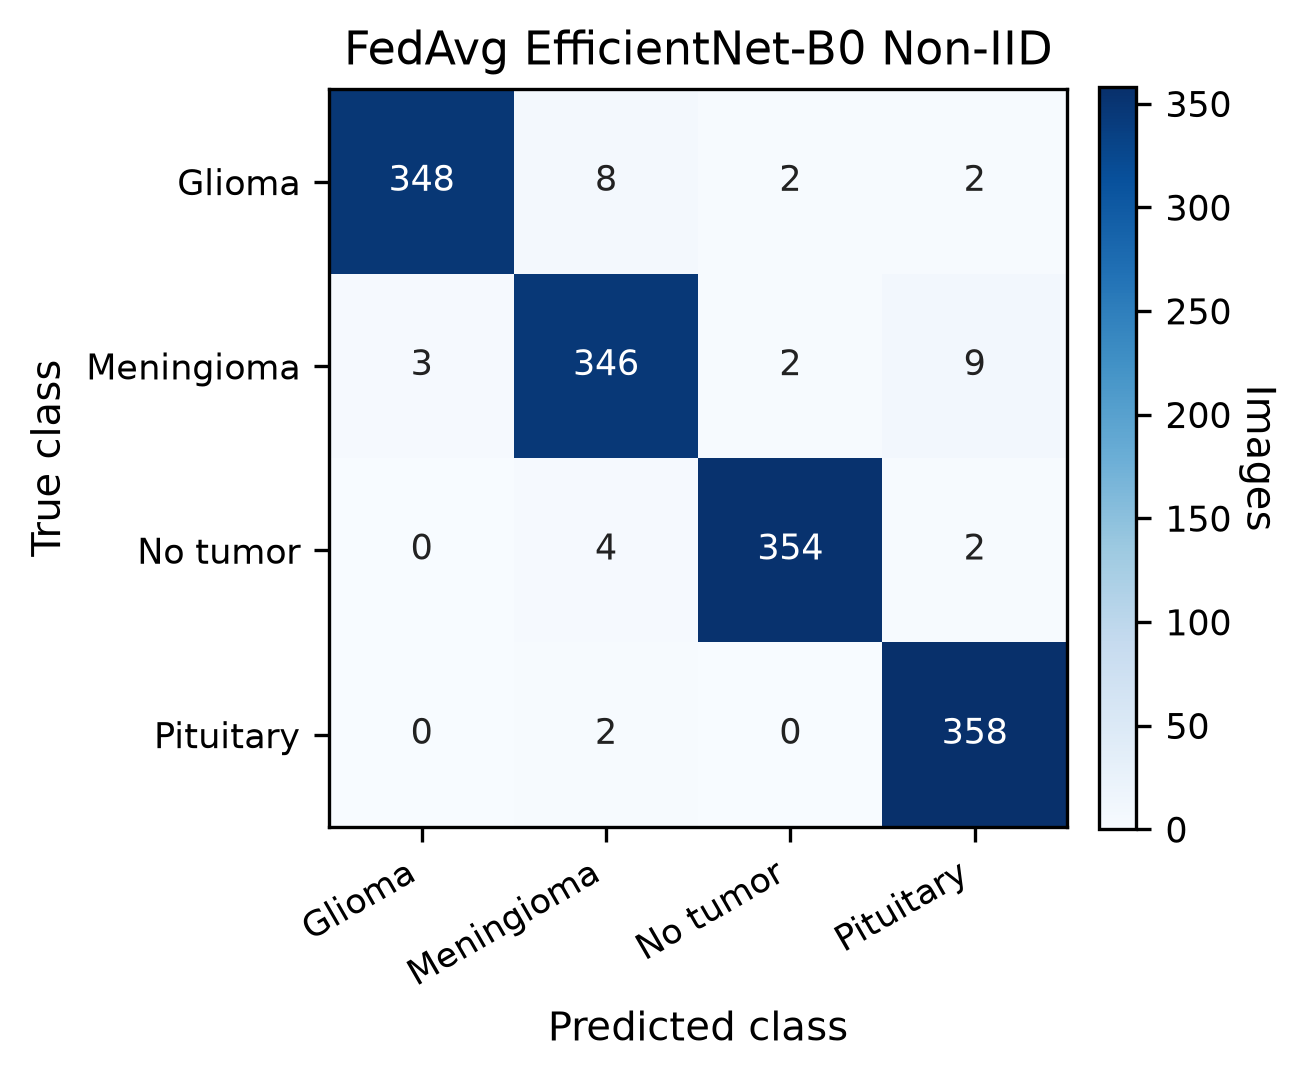
\includegraphics[width=\columnwidth]{figures/fig_confusion_matrix_efficientnet_b0_noniid.png}
\caption{Test confusion matrix for FedAvg EfficientNet-B0 under the 20-round Non-IID setting.}
\label{fig:cm}
\end{figure}

\section{Limitations}
This study is limited to a single dataset family, a single cluster-aware duplicate-controlled split, and one fixed seed. The clients are simulated from one public image collection, so the IID and 70/30 label-skew Non-IID partitions do not represent independent institutions or real cross-hospital heterogeneity \cite{naseer2026medfl,xu2023federated}. The duplicate-control procedure reduces exact, pixel-level, and conservative near-duplicate cross-split overlap, but it cannot remove all sources of dataset bias or prove patient-level independence when metadata are unavailable.

The study also lacks an independent external validation cohort, prospective evaluation, and radiologist comparison. The communication analysis measures full-state upload and download payloads, but it does not evaluate compression, secure aggregation overhead, differential privacy, encryption, network latency, packet loss, or variable client availability \cite{rieke2020future,radhika2026communication,aniket2025cfl}. Standard FL avoids centralizing raw image data in the simulated protocol, but transmitted model updates may still leak information; therefore, the results should not be interpreted as evidence of complete privacy protection or legal compliance.

\section{Conclusion}
Using a cluster-aware duplicate-controlled split and 20-round simulated FL evaluation, EfficientNet-B0 provided a favorable accuracy--communication trade-off for four-class brain tumor MRI classification. Under the same Non-IID FedAvg setting, EfficientNet-B0 achieved 97.64\% accuracy and 97.64\% macro-F1, compared with 97.22\% accuracy and 97.23\% macro-F1 for ResNet50, while reducing total communication by approximately 82.8\%. FedProx did not meaningfully improve over FedAvg in the tested configuration. Future work should evaluate independent cohorts, repeated seeds, stronger heterogeneity settings, secure aggregation, differential privacy, and communication compression.

\bibliographystyle{plain}
\bibliography{references}

\end{document}
